\chapter{Implementation}

\label{ch:implementation}

This chapter overviews the structure of the re-identification project implementation. For the detailed guide on how to use the attached software for \gls{iden} generation on a new dataset, please read \autoref{ch:guide}. For the implementation details, please refer to the attached code.

As we mentioned in the \autoref{sec:vl}, our whole work is designed as a module for \gls{VL}. Even though our work is largely independent of other modules within the framework of \gls{VL}, it shares one main component -- relation database. The database serves as an API between the modules and also as a storage for the input, output and intermediate results.

In our case, we worked with PostgreSQL as a management system. However, since we use SQLAlchemy library (\cite{sqlalchemy}) for all the communication with the database, we expect no compatibility issues with the usage of another management system.

\section{Database Structure}

As we consider the database as an \gls{api} for further processing of the data we provide quick summary of the used tables and their relations. The schema of the database is shown in \autoref{fig:database_schema}.

\begin{itemize}
    \setlength\itemsep{1em}
    \item Input tables \begin{itemize}
        \item \verb+camera+ -- basic information regarding the stream source (camera)
        \item \verb+frame+ -- record per each frame, also contains timestamp
        \item \verb+detection+ -- record per each detection, contains the image, spatial metadata and contains reference to the frame
        \item \verb+camera_setup+ -- one record per session
        \item \verb+camera_setup_assignment+ -- $n$ to $n$ mapping between \verb+camera+ and \verb+camera_setup+ tables, assigning sources to sessions
    \end{itemize}
    
    \item Intermediate results \begin{itemize}
        \item \verb+feature_type+ -- record for each type of the feature vector including hyperparameters (e.g., RGB histogram with 4 bins, or MobileNet annotator including specific setting such as description of a training set)
        \item \verb+feature_descriptor+ -- actual feature vectors for a given detection and feature type
        \item \verb+traj_model+ -- record for each type of trajectories
        \item \verb+traj+ -- record for each actual trajectory
        \item \verb+traj_detection+ -- $n$ to $n$ mapping between trajectory and detection tables for determining which detections were assigned to the trajectory
    \end{itemize}
    
    \item Output tables \begin{itemize}
        \item \verb+identity_model+ -- one record per identity model, that is specific settings, which feature type was used for the clustering, including the parameters
        \item \verb+identity+ -- record per each identity given \verb+identity_model+ created
        \item \verb+identity_detection+ -- $n$ to $n$ mapping between identity and detection tables; determining which detections were assigned to given identity
    \end{itemize}
\end{itemize}




% \begin{itemize}
%     \item camera -- contains basic information regarding the stream source
%     \item frame -- there is a record per each frame, also contains timestamp
%     \item detection -- record per each detection, contains the image, spatial metadata and contains reference to the frame
%     \item feature\_type -- there is a record for each type of the feature vector including hyperparameters (i.e. RGB hisogram with 4 bins, or MobileNet annotator including specific setting such as description of a training set)
%     \item feature\_descriptor -- these are actual feature vectors for a given detection and feature type
%     \item camera\_setup -- auxiliary table, one record per session; by the content of table camera\_setup\_assignment we can determine which cameras are part of given session
    
%     \item identity\_model -- there is one record per identity model, that is specific settings, which feature type was used for the clustering, including the parameters
%     \item identity -- auxiliary table, there is a record per each identity given identity\_model created
    
%     \item traj\_model -- same as identity\_model but for trajectories
%     \item traj -- same as identity but for trajectories
    
%     \item identity\_detection -- $n$ to $n$ mapping between identity and detection tables
%     \item traj\_detection -- $n$ to $n$ mapping between trajectory and detection tables
% \end{itemize}

\begin{figure}
    \centering
    \footnotesize
    \def\svgwidth{\columnwidth}
    %% Creator: Inkscape inkscape 0.92.3, www.inkscape.org
%% PDF/EPS/PS + LaTeX output extension by Johan Engelen, 2010
%% Accompanies image file 'database_schema.pdf' (pdf, eps, ps)
%%
%% To include the image in your LaTeX document, write
%%   \input{<filename>.pdf_tex}
%%  instead of
%%   \includegraphics{<filename>.pdf}
%% To scale the image, write
%%   \def\svgwidth{<desired width>}
%%   \input{<filename>.pdf_tex}
%%  instead of
%%   \includegraphics[width=<desired width>]{<filename>.pdf}
%%
%% Images with a different path to the parent latex file can
%% be accessed with the `import' package (which may need to be
%% installed) using
%%   \usepackage{import}
%% in the preamble, and then including the image with
%%   \import{<path to file>}{<filename>.pdf_tex}
%% Alternatively, one can specify
%%   \graphicspath{{<path to file>/}}
%% 
%% For more information, please see info/svg-inkscape on CTAN:
%%   http://tug.ctan.org/tex-archive/info/svg-inkscape
%%
\begingroup%
  \makeatletter%
  \providecommand\color[2][]{%
    \errmessage{(Inkscape) Color is used for the text in Inkscape, but the package 'color.sty' is not loaded}%
    \renewcommand\color[2][]{}%
  }%
  \providecommand\transparent[1]{%
    \errmessage{(Inkscape) Transparency is used (non-zero) for the text in Inkscape, but the package 'transparent.sty' is not loaded}%
    \renewcommand\transparent[1]{}%
  }%
  \providecommand\rotatebox[2]{#2}%
  \newcommand*\fsize{\dimexpr\f@size pt\relax}%
  \newcommand*\lineheight[1]{\fontsize{\fsize}{#1\fsize}\selectfont}%
  \ifx\svgwidth\undefined%
    \setlength{\unitlength}{555.99788482bp}%
    \ifx\svgscale\undefined%
      \relax%
    \else%
      \setlength{\unitlength}{\unitlength * \real{\svgscale}}%
    \fi%
  \else%
    \setlength{\unitlength}{\svgwidth}%
  \fi%
  \global\let\svgwidth\undefined%
  \global\let\svgscale\undefined%
  \makeatother%
  \begin{picture}(1,1.17981813)%
    \lineheight{1}%
    \setlength\tabcolsep{0pt}%
    \put(0,0){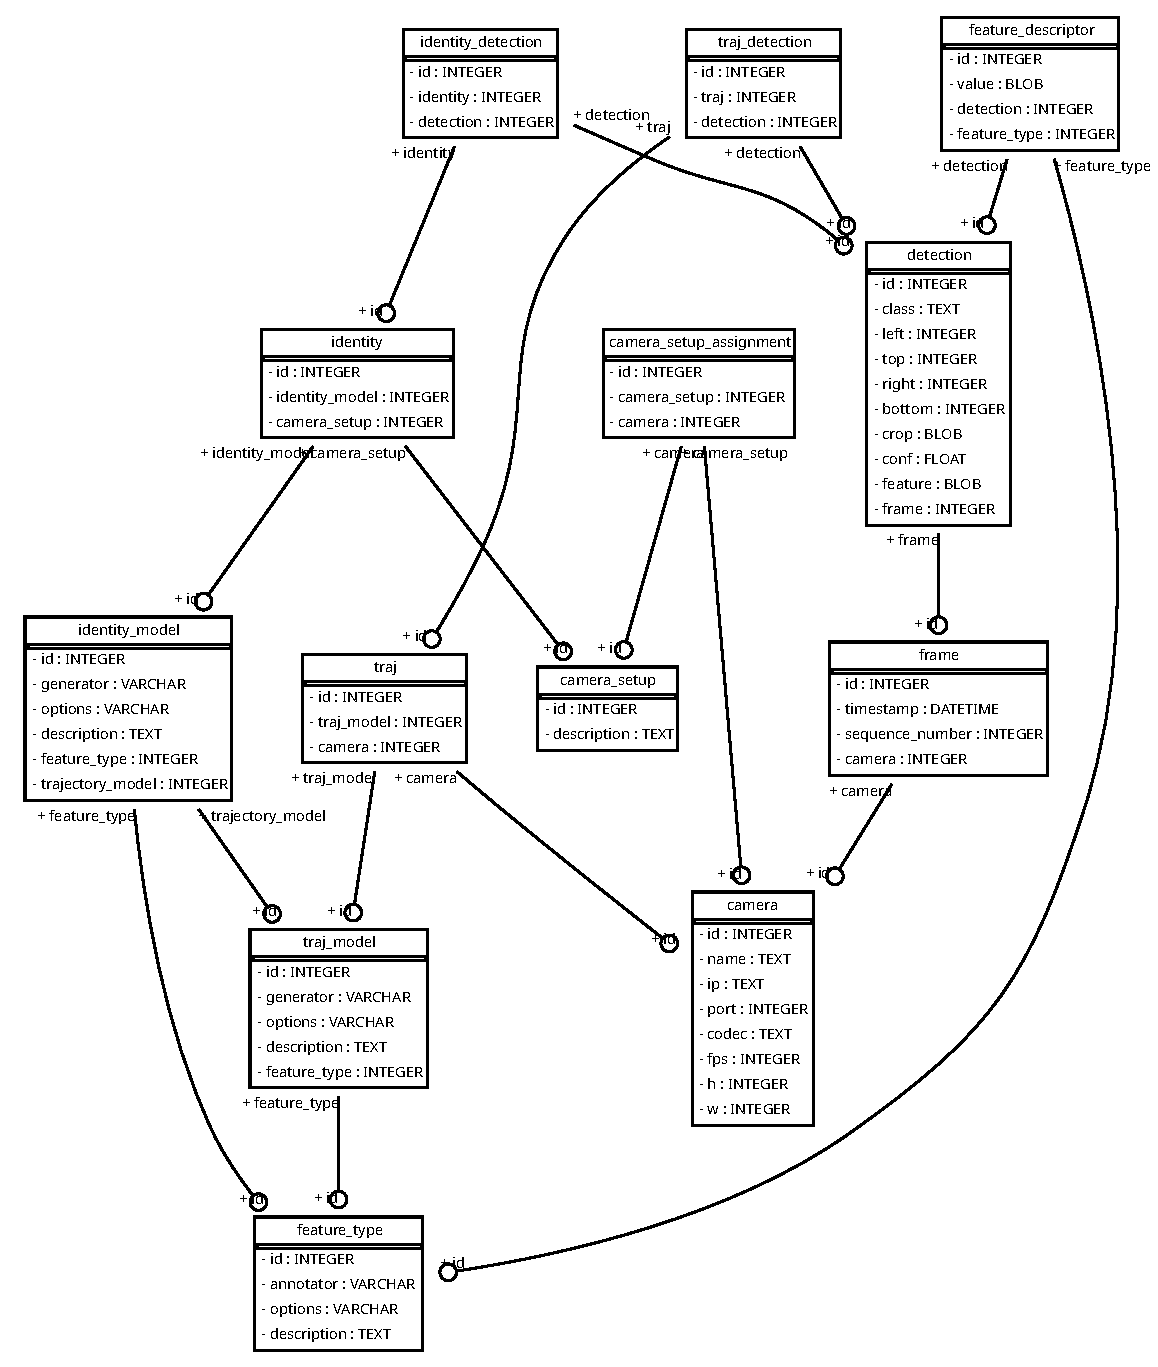
\includegraphics[width=\unitlength,page=1]{database_schema.pdf}}%
    \put(0.62767763,0.3945916){\color[rgb]{0,0,0}\makebox(0,0)[lt]{\lineheight{1.25}\smash{\begin{tabular}[t]{l}camera\end{tabular}}}}%
    \put(0,0){\includegraphics[width=\unitlength,page=2]{database_schema.pdf}}%
    \put(0.60339784,0.36941256){\color[rgb]{0,0,0}\makebox(0,0)[lt]{\lineheight{1.25}\smash{\begin{tabular}[t]{l}- id : INTEGER\end{tabular}}}}%
    \put(0.60339784,0.34783052){\color[rgb]{0,0,0}\makebox(0,0)[lt]{\lineheight{1.25}\smash{\begin{tabular}[t]{l}- name : TEXT\end{tabular}}}}%
    \put(0.60339784,0.32624848){\color[rgb]{0,0,0}\makebox(0,0)[lt]{\lineheight{1.25}\smash{\begin{tabular}[t]{l}- ip : TEXT\end{tabular}}}}%
    \put(0.60339784,0.30466644){\color[rgb]{0,0,0}\makebox(0,0)[lt]{\lineheight{1.25}\smash{\begin{tabular}[t]{l}- port : INTEGER\end{tabular}}}}%
    \put(0.60339784,0.2830844){\color[rgb]{0,0,0}\makebox(0,0)[lt]{\lineheight{1.25}\smash{\begin{tabular}[t]{l}- codec : TEXT\end{tabular}}}}%
    \put(0.60339784,0.26150236){\color[rgb]{0,0,0}\makebox(0,0)[lt]{\lineheight{1.25}\smash{\begin{tabular}[t]{l}- fps : INTEGER\end{tabular}}}}%
    \put(0.60339784,0.23992032){\color[rgb]{0,0,0}\makebox(0,0)[lt]{\lineheight{1.25}\smash{\begin{tabular}[t]{l}- h : INTEGER\end{tabular}}}}%
    \put(0.60339784,0.2183383){\color[rgb]{0,0,0}\makebox(0,0)[lt]{\lineheight{1.25}\smash{\begin{tabular}[t]{l}- w : INTEGER\end{tabular}}}}%
    \put(0,0){\includegraphics[width=\unitlength,page=3]{database_schema.pdf}}%
    \put(0.79313993,0.61041199){\color[rgb]{0,0,0}\makebox(0,0)[lt]{\lineheight{1.25}\smash{\begin{tabular}[t]{l}frame\end{tabular}}}}%
    \put(0,0){\includegraphics[width=\unitlength,page=4]{database_schema.pdf}}%
    \put(0.72209905,0.58523295){\color[rgb]{0,0,0}\makebox(0,0)[lt]{\lineheight{1.25}\smash{\begin{tabular}[t]{l}- id : INTEGER\end{tabular}}}}%
    \put(0.72209905,0.56365091){\color[rgb]{0,0,0}\makebox(0,0)[lt]{\lineheight{1.25}\smash{\begin{tabular}[t]{l}- timestamp : DATETIME\end{tabular}}}}%
    \put(0.72209905,0.54206887){\color[rgb]{0,0,0}\makebox(0,0)[lt]{\lineheight{1.25}\smash{\begin{tabular}[t]{l}- sequence\_number : INTEGER\end{tabular}}}}%
    \put(0.72209905,0.52048683){\color[rgb]{0,0,0}\makebox(0,0)[lt]{\lineheight{1.25}\smash{\begin{tabular}[t]{l}- camera : INTEGER\end{tabular}}}}%
    \put(0,0){\includegraphics[width=\unitlength,page=5]{database_schema.pdf}}%
    \put(0.70621467,0.42181537){\color[rgb]{0,0,0}\makebox(0,0)[t]{\lineheight{1.25}\smash{\begin{tabular}[t]{c}+ id\end{tabular}}}}%
    \put(0.74285649,0.49290268){\color[rgb]{0,0,0}\makebox(0,0)[t]{\lineheight{1.25}\smash{\begin{tabular}[t]{c}+ camera\end{tabular}}}}%
    \put(0.78324817,0.95572467){\color[rgb]{0,0,0}\makebox(0,0)[lt]{\lineheight{1.25}\smash{\begin{tabular}[t]{l}detection\end{tabular}}}}%
    \put(0,0){\includegraphics[width=\unitlength,page=6]{database_schema.pdf}}%
    \put(0.75447211,0.93054563){\color[rgb]{0,0,0}\makebox(0,0)[lt]{\lineheight{1.25}\smash{\begin{tabular}[t]{l}- id : INTEGER\end{tabular}}}}%
    \put(0.75447211,0.90896353){\color[rgb]{0,0,0}\makebox(0,0)[lt]{\lineheight{1.25}\smash{\begin{tabular}[t]{l}- class : TEXT\end{tabular}}}}%
    \put(0.75447211,0.88738149){\color[rgb]{0,0,0}\makebox(0,0)[lt]{\lineheight{1.25}\smash{\begin{tabular}[t]{l}- left : INTEGER\end{tabular}}}}%
    \put(0.75447211,0.86579945){\color[rgb]{0,0,0}\makebox(0,0)[lt]{\lineheight{1.25}\smash{\begin{tabular}[t]{l}- top : INTEGER\end{tabular}}}}%
    \put(0.75447211,0.84421741){\color[rgb]{0,0,0}\makebox(0,0)[lt]{\lineheight{1.25}\smash{\begin{tabular}[t]{l}- right : INTEGER\end{tabular}}}}%
    \put(0.75447211,0.82263538){\color[rgb]{0,0,0}\makebox(0,0)[lt]{\lineheight{1.25}\smash{\begin{tabular}[t]{l}- bottom : INTEGER\end{tabular}}}}%
    \put(0.75447211,0.80105334){\color[rgb]{0,0,0}\makebox(0,0)[lt]{\lineheight{1.25}\smash{\begin{tabular}[t]{l}- crop : BLOB\end{tabular}}}}%
    \put(0.75447211,0.7794713){\color[rgb]{0,0,0}\makebox(0,0)[lt]{\lineheight{1.25}\smash{\begin{tabular}[t]{l}- conf : FLOAT\end{tabular}}}}%
    \put(0.75447211,0.75788926){\color[rgb]{0,0,0}\makebox(0,0)[lt]{\lineheight{1.25}\smash{\begin{tabular}[t]{l}- feature : BLOB\end{tabular}}}}%
    \put(0.75447211,0.73630722){\color[rgb]{0,0,0}\makebox(0,0)[lt]{\lineheight{1.25}\smash{\begin{tabular}[t]{l}- frame : INTEGER\end{tabular}}}}%
    \put(0,0){\includegraphics[width=\unitlength,page=7]{database_schema.pdf}}%
    \put(0.79943469,0.63751759){\color[rgb]{0,0,0}\makebox(0,0)[t]{\lineheight{1.25}\smash{\begin{tabular}[t]{c}+ id\end{tabular}}}}%
    \put(0.78774442,0.70921512){\color[rgb]{0,0,0}\makebox(0,0)[t]{\lineheight{1.25}\smash{\begin{tabular}[t]{c}+ frame\end{tabular}}}}%
    \put(0.25628671,0.11402511){\color[rgb]{0,0,0}\makebox(0,0)[lt]{\lineheight{1.25}\smash{\begin{tabular}[t]{l}feature\_type\end{tabular}}}}%
    \put(0,0){\includegraphics[width=\unitlength,page=8]{database_schema.pdf}}%
    \put(0.22571216,0.08884606){\color[rgb]{0,0,0}\makebox(0,0)[lt]{\lineheight{1.25}\smash{\begin{tabular}[t]{l}- id : INTEGER\end{tabular}}}}%
    \put(0.22571216,0.06726402){\color[rgb]{0,0,0}\makebox(0,0)[lt]{\lineheight{1.25}\smash{\begin{tabular}[t]{l}- annotator : VARCHAR\end{tabular}}}}%
    \put(0.22571216,0.04568198){\color[rgb]{0,0,0}\makebox(0,0)[lt]{\lineheight{1.25}\smash{\begin{tabular}[t]{l}- options : VARCHAR\end{tabular}}}}%
    \put(0.22571216,0.02409994){\color[rgb]{0,0,0}\makebox(0,0)[lt]{\lineheight{1.25}\smash{\begin{tabular}[t]{l}- description : TEXT\end{tabular}}}}%
    \put(0,0){\includegraphics[width=\unitlength,page=9]{database_schema.pdf}}%
    \put(0.83630401,1.14996302){\color[rgb]{0,0,0}\makebox(0,0)[lt]{\lineheight{1.25}\smash{\begin{tabular}[t]{l}feature\_descriptor\end{tabular}}}}%
    \put(0,0){\includegraphics[width=\unitlength,page=10]{database_schema.pdf}}%
    \put(0.81921823,1.12478398){\color[rgb]{0,0,0}\makebox(0,0)[lt]{\lineheight{1.25}\smash{\begin{tabular}[t]{l}- id : INTEGER\end{tabular}}}}%
    \put(0.81921823,1.10320194){\color[rgb]{0,0,0}\makebox(0,0)[lt]{\lineheight{1.25}\smash{\begin{tabular}[t]{l}- value : BLOB\end{tabular}}}}%
    \put(0.81921823,1.0816199){\color[rgb]{0,0,0}\makebox(0,0)[lt]{\lineheight{1.25}\smash{\begin{tabular}[t]{l}- detection : INTEGER\end{tabular}}}}%
    \put(0.81921823,1.06003786){\color[rgb]{0,0,0}\makebox(0,0)[lt]{\lineheight{1.25}\smash{\begin{tabular}[t]{l}- feature\_type : INTEGER\end{tabular}}}}%
    \put(0,0){\includegraphics[width=\unitlength,page=11]{database_schema.pdf}}%
    \put(0.83915391,0.98320014){\color[rgb]{0,0,0}\makebox(0,0)[t]{\lineheight{1.25}\smash{\begin{tabular}[t]{c}+ id\end{tabular}}}}%
    \put(0.83701786,1.0324536){\color[rgb]{0,0,0}\makebox(0,0)[t]{\lineheight{1.25}\smash{\begin{tabular}[t]{c}+ detection\end{tabular}}}}%
    \put(0,0){\includegraphics[width=\unitlength,page=12]{database_schema.pdf}}%
    \put(0.39062033,0.08506201){\color[rgb]{0,0,0}\makebox(0,0)[t]{\lineheight{1.25}\smash{\begin{tabular}[t]{c}+ id\end{tabular}}}}%
    \put(0.95144038,1.03281113){\color[rgb]{0,0,0}\makebox(0,0)[t]{\lineheight{1.25}\smash{\begin{tabular}[t]{c}+ feature\_type\end{tabular}}}}%
    \put(0.26168222,0.36221854){\color[rgb]{0,0,0}\makebox(0,0)[lt]{\lineheight{1.25}\smash{\begin{tabular}[t]{l}traj\_model\end{tabular}}}}%
    \put(0,0){\includegraphics[width=\unitlength,page=13]{database_schema.pdf}}%
    \put(0.22211515,0.3370395){\color[rgb]{0,0,0}\makebox(0,0)[lt]{\lineheight{1.25}\smash{\begin{tabular}[t]{l}- id : INTEGER\end{tabular}}}}%
    \put(0.22211515,0.31545746){\color[rgb]{0,0,0}\makebox(0,0)[lt]{\lineheight{1.25}\smash{\begin{tabular}[t]{l}- generator : VARCHAR\end{tabular}}}}%
    \put(0.22211515,0.29387542){\color[rgb]{0,0,0}\makebox(0,0)[lt]{\lineheight{1.25}\smash{\begin{tabular}[t]{l}- options : VARCHAR\end{tabular}}}}%
    \put(0.22211515,0.27229338){\color[rgb]{0,0,0}\makebox(0,0)[lt]{\lineheight{1.25}\smash{\begin{tabular}[t]{l}- description : TEXT\end{tabular}}}}%
    \put(0.22211515,0.25071134){\color[rgb]{0,0,0}\makebox(0,0)[lt]{\lineheight{1.25}\smash{\begin{tabular}[t]{l}- feature\_type : INTEGER\end{tabular}}}}%
    \put(0,0){\includegraphics[width=\unitlength,page=14]{database_schema.pdf}}%
    \put(0.28146576,0.14172187){\color[rgb]{0,0,0}\makebox(0,0)[t]{\lineheight{1.25}\smash{\begin{tabular}[t]{c}+ id\end{tabular}}}}%
    \put(0.2508912,0.2235027){\color[rgb]{0,0,0}\makebox(0,0)[t]{\lineheight{1.25}\smash{\begin{tabular}[t]{c}+ feature\_type\end{tabular}}}}%
    \put(0.32283133,0.59962097){\color[rgb]{0,0,0}\makebox(0,0)[lt]{\lineheight{1.25}\smash{\begin{tabular}[t]{l}traj\end{tabular}}}}%
    \put(0,0){\includegraphics[width=\unitlength,page=15]{database_schema.pdf}}%
    \put(0.26707773,0.57444193){\color[rgb]{0,0,0}\makebox(0,0)[lt]{\lineheight{1.25}\smash{\begin{tabular}[t]{l}- id : INTEGER\end{tabular}}}}%
    \put(0.26707773,0.55285989){\color[rgb]{0,0,0}\makebox(0,0)[lt]{\lineheight{1.25}\smash{\begin{tabular}[t]{l}- traj\_model : INTEGER\end{tabular}}}}%
    \put(0.26707773,0.53127785){\color[rgb]{0,0,0}\makebox(0,0)[lt]{\lineheight{1.25}\smash{\begin{tabular}[t]{l}- camera : INTEGER\end{tabular}}}}%
    \put(0,0){\includegraphics[width=\unitlength,page=16]{database_schema.pdf}}%
    \put(0.57265583,0.36552636){\color[rgb]{0,0,0}\makebox(0,0)[t]{\lineheight{1.25}\smash{\begin{tabular}[t]{c}+ id\end{tabular}}}}%
    \put(0.3673941,0.50400534){\color[rgb]{0,0,0}\makebox(0,0)[t]{\lineheight{1.25}\smash{\begin{tabular}[t]{c}+ camera\end{tabular}}}}%
    \put(0,0){\includegraphics[width=\unitlength,page=17]{database_schema.pdf}}%
    \put(0.29305065,0.38948765){\color[rgb]{0,0,0}\makebox(0,0)[t]{\lineheight{1.25}\smash{\begin{tabular}[t]{c}+ id\end{tabular}}}}%
    \put(0.28755928,0.50396379){\color[rgb]{0,0,0}\makebox(0,0)[t]{\lineheight{1.25}\smash{\begin{tabular}[t]{c}+ traj\_model\end{tabular}}}}%
    \put(0.61958437,1.139172){\color[rgb]{0,0,0}\makebox(0,0)[lt]{\lineheight{1.25}\smash{\begin{tabular}[t]{l}traj\_detection\end{tabular}}}}%
    \put(0,0){\includegraphics[width=\unitlength,page=18]{database_schema.pdf}}%
    \put(0.59800233,1.11399296){\color[rgb]{0,0,0}\makebox(0,0)[lt]{\lineheight{1.25}\smash{\begin{tabular}[t]{l}- id : INTEGER\end{tabular}}}}%
    \put(0.59800233,1.09241092){\color[rgb]{0,0,0}\makebox(0,0)[lt]{\lineheight{1.25}\smash{\begin{tabular}[t]{l}- traj : INTEGER\end{tabular}}}}%
    \put(0.59800233,1.07082888){\color[rgb]{0,0,0}\makebox(0,0)[lt]{\lineheight{1.25}\smash{\begin{tabular}[t]{l}- detection : INTEGER\end{tabular}}}}%
    \put(0,0){\includegraphics[width=\unitlength,page=19]{database_schema.pdf}}%
    \put(0.7236105,0.98319422){\color[rgb]{0,0,0}\makebox(0,0)[t]{\lineheight{1.25}\smash{\begin{tabular}[t]{c}+ id\end{tabular}}}}%
    \put(0.65844857,1.04351477){\color[rgb]{0,0,0}\makebox(0,0)[t]{\lineheight{1.25}\smash{\begin{tabular}[t]{c}+ detection\end{tabular}}}}%
    \put(0,0){\includegraphics[width=\unitlength,page=20]{database_schema.pdf}}%
    \put(0.35820125,0.62665862){\color[rgb]{0,0,0}\makebox(0,0)[t]{\lineheight{1.25}\smash{\begin{tabular}[t]{c}+ id\end{tabular}}}}%
    \put(0.56364877,1.06631495){\color[rgb]{0,0,0}\makebox(0,0)[t]{\lineheight{1.25}\smash{\begin{tabular}[t]{c}+ traj\end{tabular}}}}%
    \put(0.48379737,0.58882995){\color[rgb]{0,0,0}\makebox(0,0)[lt]{\lineheight{1.25}\smash{\begin{tabular}[t]{l}camera\_setup\end{tabular}}}}%
    \put(0,0){\includegraphics[width=\unitlength,page=21]{database_schema.pdf}}%
    \put(0.4703086,0.56365091){\color[rgb]{0,0,0}\makebox(0,0)[lt]{\lineheight{1.25}\smash{\begin{tabular}[t]{l}- id : INTEGER\end{tabular}}}}%
    \put(0.4703086,0.54206887){\color[rgb]{0,0,0}\makebox(0,0)[lt]{\lineheight{1.25}\smash{\begin{tabular}[t]{l}- description : TEXT\end{tabular}}}}%
    \put(0,0){\includegraphics[width=\unitlength,page=22]{database_schema.pdf}}%
    \put(0.5260622,0.88018748){\color[rgb]{0,0,0}\makebox(0,0)[lt]{\lineheight{1.25}\smash{\begin{tabular}[t]{l}camera\_setup\_assignment\end{tabular}}}}%
    \put(0,0){\includegraphics[width=\unitlength,page=23]{database_schema.pdf}}%
    \put(0.5260622,0.85500843){\color[rgb]{0,0,0}\makebox(0,0)[lt]{\lineheight{1.25}\smash{\begin{tabular}[t]{l}- id : INTEGER\end{tabular}}}}%
    \put(0.5260622,0.83342639){\color[rgb]{0,0,0}\makebox(0,0)[lt]{\lineheight{1.25}\smash{\begin{tabular}[t]{l}- camera\_setup : INTEGER\end{tabular}}}}%
    \put(0.5260622,0.81184436){\color[rgb]{0,0,0}\makebox(0,0)[lt]{\lineheight{1.25}\smash{\begin{tabular}[t]{l}- camera : INTEGER\end{tabular}}}}%
    \put(0,0){\includegraphics[width=\unitlength,page=24]{database_schema.pdf}}%
    \put(0.6300087,0.42165082){\color[rgb]{0,0,0}\makebox(0,0)[t]{\lineheight{1.25}\smash{\begin{tabular}[t]{c}+ id\end{tabular}}}}%
    \put(0.58111798,0.78461735){\color[rgb]{0,0,0}\makebox(0,0)[t]{\lineheight{1.25}\smash{\begin{tabular}[t]{c}+ camera\end{tabular}}}}%
    \put(0,0){\includegraphics[width=\unitlength,page=25]{database_schema.pdf}}%
    \put(0.52582658,0.61644347){\color[rgb]{0,0,0}\makebox(0,0)[t]{\lineheight{1.25}\smash{\begin{tabular}[t]{c}+ id\end{tabular}}}}%
    \put(0.63400187,0.78472581){\color[rgb]{0,0,0}\makebox(0,0)[t]{\lineheight{1.25}\smash{\begin{tabular}[t]{c}+ camera\_setup\end{tabular}}}}%
    \put(0.06744387,0.63199403){\color[rgb]{0,0,0}\makebox(0,0)[lt]{\lineheight{1.25}\smash{\begin{tabular}[t]{l}identity\_model\end{tabular}}}}%
    \put(0,0){\includegraphics[width=\unitlength,page=26]{database_schema.pdf}}%
    \put(0.0278768,0.60681499){\color[rgb]{0,0,0}\makebox(0,0)[lt]{\lineheight{1.25}\smash{\begin{tabular}[t]{l}- id : INTEGER\end{tabular}}}}%
    \put(0.0278768,0.58523295){\color[rgb]{0,0,0}\makebox(0,0)[lt]{\lineheight{1.25}\smash{\begin{tabular}[t]{l}- generator : VARCHAR\end{tabular}}}}%
    \put(0.0278768,0.56365091){\color[rgb]{0,0,0}\makebox(0,0)[lt]{\lineheight{1.25}\smash{\begin{tabular}[t]{l}- options : VARCHAR\end{tabular}}}}%
    \put(0.0278768,0.54206887){\color[rgb]{0,0,0}\makebox(0,0)[lt]{\lineheight{1.25}\smash{\begin{tabular}[t]{l}- description : TEXT\end{tabular}}}}%
    \put(0.0278768,0.52048683){\color[rgb]{0,0,0}\makebox(0,0)[lt]{\lineheight{1.25}\smash{\begin{tabular}[t]{l}- feature\_type : INTEGER\end{tabular}}}}%
    \put(0.0278768,0.49890479){\color[rgb]{0,0,0}\makebox(0,0)[lt]{\lineheight{1.25}\smash{\begin{tabular}[t]{l}- trajectory\_model : INTEGER\end{tabular}}}}%
    \put(0,0){\includegraphics[width=\unitlength,page=27]{database_schema.pdf}}%
    \put(0.21684824,0.14102442){\color[rgb]{0,0,0}\makebox(0,0)[t]{\lineheight{1.25}\smash{\begin{tabular}[t]{c}+ id\end{tabular}}}}%
    \put(0.07459994,0.47141071){\color[rgb]{0,0,0}\makebox(0,0)[t]{\lineheight{1.25}\smash{\begin{tabular}[t]{c}+ feature\_type\end{tabular}}}}%
    \put(0,0){\includegraphics[width=\unitlength,page=28]{database_schema.pdf}}%
    \put(0.22824211,0.38954215){\color[rgb]{0,0,0}\makebox(0,0)[t]{\lineheight{1.25}\smash{\begin{tabular}[t]{c}+ id\end{tabular}}}}%
    \put(0.22645404,0.47129688){\color[rgb]{0,0,0}\makebox(0,0)[t]{\lineheight{1.25}\smash{\begin{tabular}[t]{c}+ trajectory\_model\end{tabular}}}}%
    \put(0.28596202,0.88018748){\color[rgb]{0,0,0}\makebox(0,0)[lt]{\lineheight{1.25}\smash{\begin{tabular}[t]{l}identity\end{tabular}}}}%
    \put(0,0){\includegraphics[width=\unitlength,page=29]{database_schema.pdf}}%
    \put(0.23110767,0.85500843){\color[rgb]{0,0,0}\makebox(0,0)[lt]{\lineheight{1.25}\smash{\begin{tabular}[t]{l}- id : INTEGER\end{tabular}}}}%
    \put(0.23110767,0.83342639){\color[rgb]{0,0,0}\makebox(0,0)[lt]{\lineheight{1.25}\smash{\begin{tabular}[t]{l}- identity\_model : INTEGER\end{tabular}}}}%
    \put(0.23110767,0.81184436){\color[rgb]{0,0,0}\makebox(0,0)[lt]{\lineheight{1.25}\smash{\begin{tabular}[t]{l}- camera\_setup : INTEGER\end{tabular}}}}%
    \put(0,0){\includegraphics[width=\unitlength,page=30]{database_schema.pdf}}%
    \put(0.47978044,0.61644347){\color[rgb]{0,0,0}\makebox(0,0)[t]{\lineheight{1.25}\smash{\begin{tabular}[t]{c}+ id\end{tabular}}}}%
    \put(0.30419382,0.78472581){\color[rgb]{0,0,0}\makebox(0,0)[t]{\lineheight{1.25}\smash{\begin{tabular}[t]{c}+ camera\_setup\end{tabular}}}}%
    \put(0,0){\includegraphics[width=\unitlength,page=31]{database_schema.pdf}}%
    \put(0.16080525,0.65913596){\color[rgb]{0,0,0}\makebox(0,0)[t]{\lineheight{1.25}\smash{\begin{tabular}[t]{c}+ id\end{tabular}}}}%
    \put(0.22173909,0.78472581){\color[rgb]{0,0,0}\makebox(0,0)[t]{\lineheight{1.25}\smash{\begin{tabular}[t]{c}+ identity\_model\end{tabular}}}}%
    \put(0.3623984,1.139172){\color[rgb]{0,0,0}\makebox(0,0)[lt]{\lineheight{1.25}\smash{\begin{tabular}[t]{l}identity\_detection\end{tabular}}}}%
    \put(0,0){\includegraphics[width=\unitlength,page=32]{database_schema.pdf}}%
    \put(0.35340589,1.11399296){\color[rgb]{0,0,0}\makebox(0,0)[lt]{\lineheight{1.25}\smash{\begin{tabular}[t]{l}- id : INTEGER\end{tabular}}}}%
    \put(0.35340589,1.09241092){\color[rgb]{0,0,0}\makebox(0,0)[lt]{\lineheight{1.25}\smash{\begin{tabular}[t]{l}- identity : INTEGER\end{tabular}}}}%
    \put(0.35340589,1.07082888){\color[rgb]{0,0,0}\makebox(0,0)[lt]{\lineheight{1.25}\smash{\begin{tabular}[t]{l}- detection : INTEGER\end{tabular}}}}%
    \put(0,0){\includegraphics[width=\unitlength,page=33]{database_schema.pdf}}%
    \put(0.72289276,0.96751077){\color[rgb]{0,0,0}\makebox(0,0)[t]{\lineheight{1.25}\smash{\begin{tabular}[t]{c}+ id\end{tabular}}}}%
    \put(0.52795549,1.07632187){\color[rgb]{0,0,0}\makebox(0,0)[t]{\lineheight{1.25}\smash{\begin{tabular}[t]{c}+ detection\end{tabular}}}}%
    \put(0,0){\includegraphics[width=\unitlength,page=34]{database_schema.pdf}}%
    \put(0.31986757,0.90743013){\color[rgb]{0,0,0}\makebox(0,0)[t]{\lineheight{1.25}\smash{\begin{tabular}[t]{c}+ id\end{tabular}}}}%
    \put(0.36533302,1.04351477){\color[rgb]{0,0,0}\makebox(0,0)[t]{\lineheight{1.25}\smash{\begin{tabular}[t]{c}+ identity\end{tabular}}}}%
  \end{picture}%
\endgroup%

    \caption[Schema of the database]{Schema of the database. The connections represent foreign keys connecting the tables. The name of the foreign key is always the same as the name of the table it references. It always references the primary key -- column \texttt{id}.}
    \label{fig:database_schema}
\end{figure}

\section{Code Structure}
The implementation is split into several parts. Each part is largely independent of the others, using only the database as the common point (similarly to \gls{VL} modules). For the purpose of testing and evaluation, we also add a command-line interface for each part.  Alongside the parts, which we describe further in more detail, we also provide several small scripts used for the evaluation.

The first part -- feature vector extractor -- is responsible for creating feature vectors described in \autoref{ch:features}. The main pipeline for this module consists of downloading the data to compute the feature vectors from the database, annotate them with the feature vectors, and then upload the results back to the database. If we use annotators that are based on the \gls{nn}, the model needs to be trained first. In this case the data for training is firstly downloaded and used to train the network. Then we run the annotation process as described in the main pipeline with the trained network. For any subsequent annotation with the same setting the locally stored network is used instead of training the network again.

The second part -- clustering part -- is responsible for clustering the \glspl{det} (\autoref{ch:iden_construction}), that is for both -- trajectory generation and identity generation. For this process, the \glspl{det} from given cameras are again retrieved from the database along, if applicable, with the corresponding feature vectors created with the selected settings. If we cluster the \glspl{det} based on a priory created trajectories, these trajectories are also queried. Once the \glspl{det} are clustered according to the parameters, the resulting trajectories or \glspl{iden} are again committed to the database for use by other \gls{VL} modules. The options which were supplied for the \gls{iden} construction is also committed to the database as a new ``\gls{iden} model''. All the created \glspl{iden} are assigned to this model so they can be later queried if the same options are supplied.


\section{Annotation Tool}
We also provide a tool for manual annotation of the \glspl{det} we used to obtain the ground truth for our datasets. The tool queries the \glspl{det} from the database as well as selected \glspl{iden} or trajectory. User then can see the \glspl{det} frame-by-frame as well as their division to \glspl{iden}. It is possible to re-assign the \glspl{det} to different \gls{iden}. This approach allows for semi-automated annotation: The \glspl{det} are firstly clustered by a (even poor) algorithm, then only wrongly assigned \glspl{det} need to be corrected. Once the re-assignment is complete, the resulting clustering can be committed back to the database as a new set of \glspl{iden} with a new ``identity model''. A screenshot of the tool is in \autoref{fig:annotation_tool}.

\begin{figure}
    \centering
    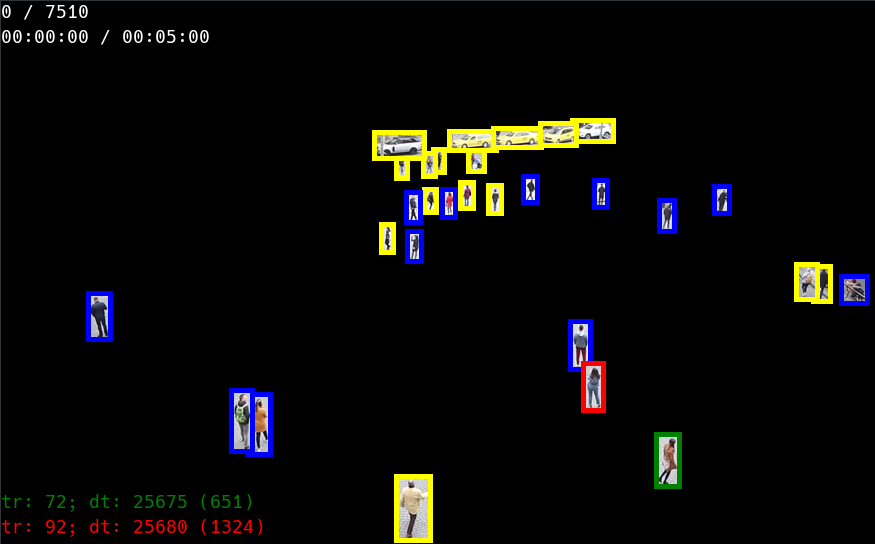
\includegraphics[width=\textwidth]{img/annotator_screenshot.png}
    \caption{Screenshot of the annotation tool}
    \label{fig:annotation_tool}
\end{figure}
